\section{Experimental Evaluation}

\begin{figure}[tb]
    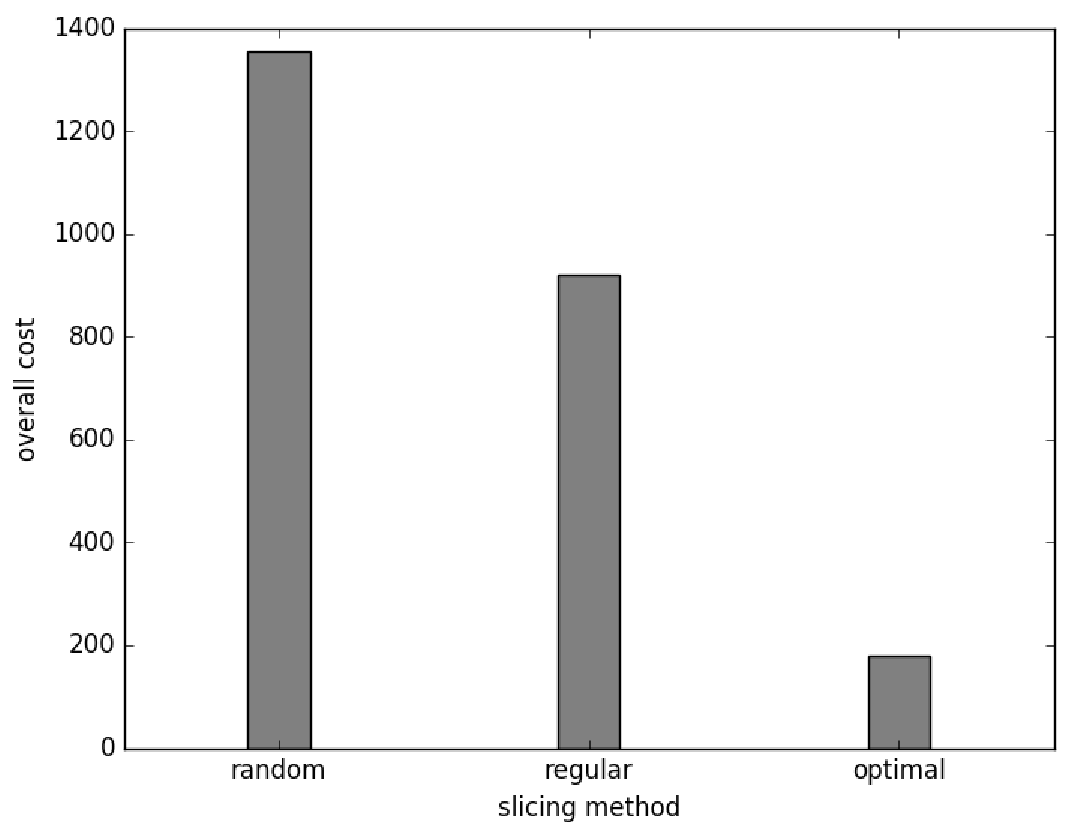
\includegraphics[width=3in]{figs/cuts_cost.pdf}
    \caption{Relative query answering cost}
\end{figure}

\begin{figure}[tb]
    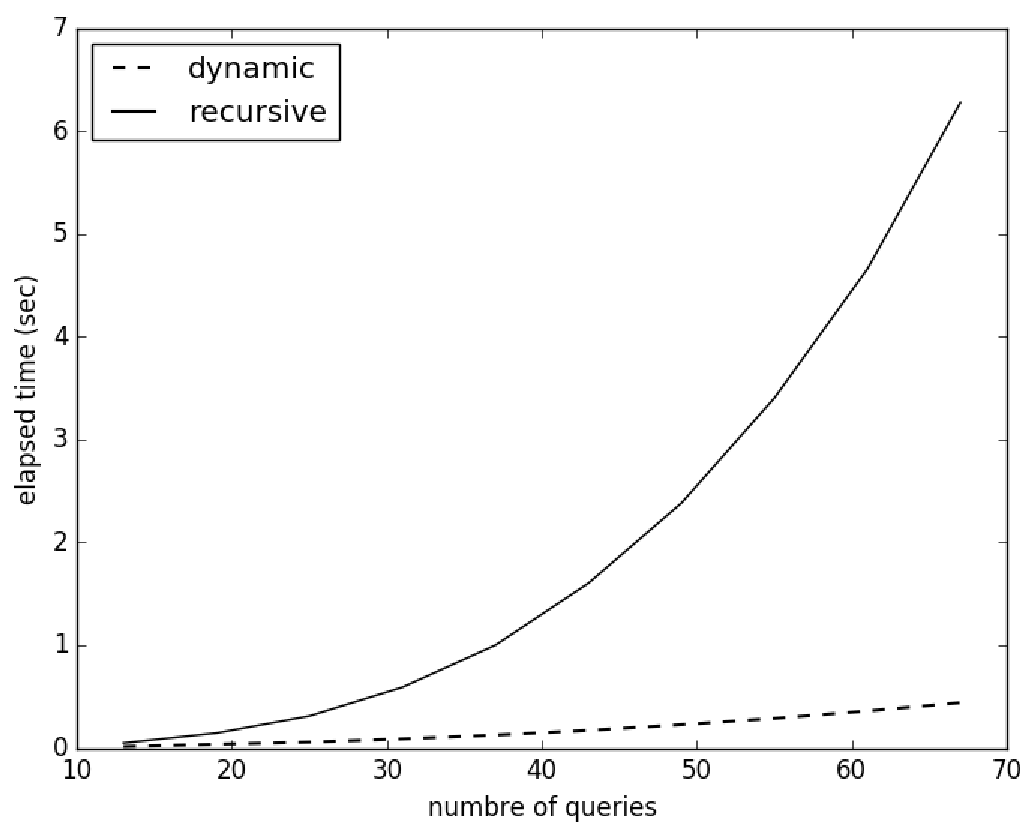
\includegraphics[width=3in]{figs/multiquery_runtime.pdf}
    \caption{Optimization time with respect to the number of queries}
\end{figure}

\begin{figure}[tb]
    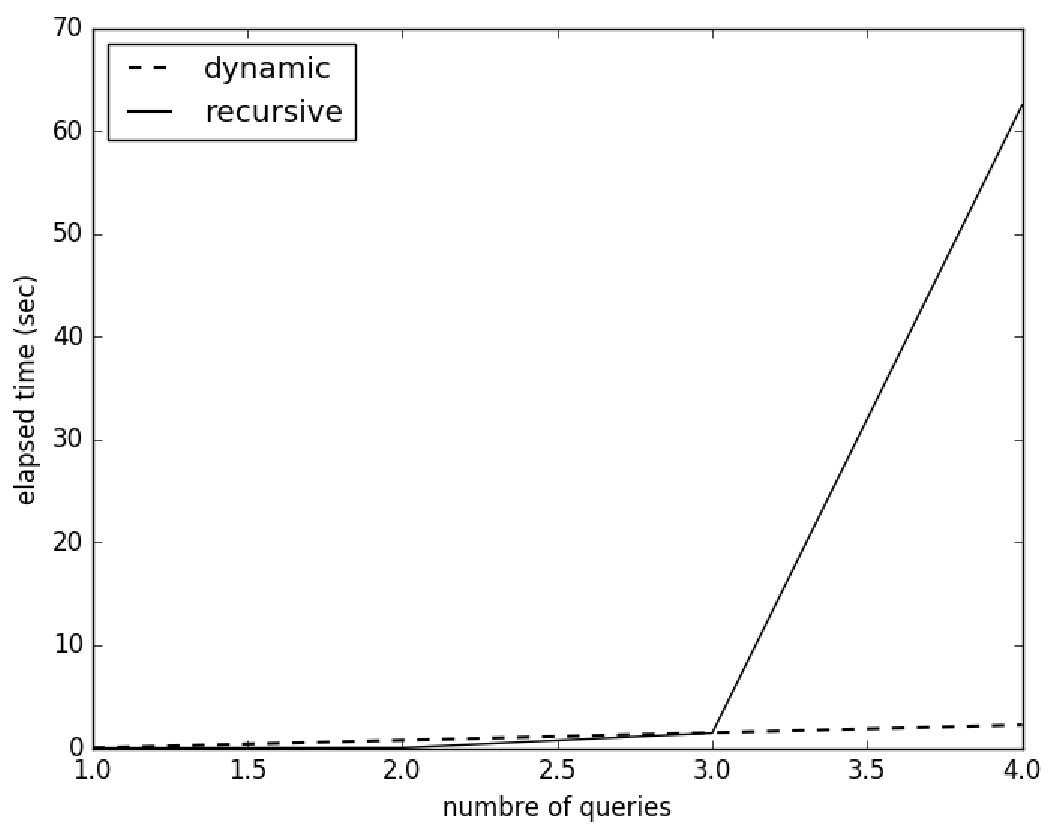
\includegraphics[width=3in]{figs/multisnap_runtime.pdf}
    \caption{Optimization time with respect to the number of snapshots}
\end{figure}

\begin{figure}[tb]
    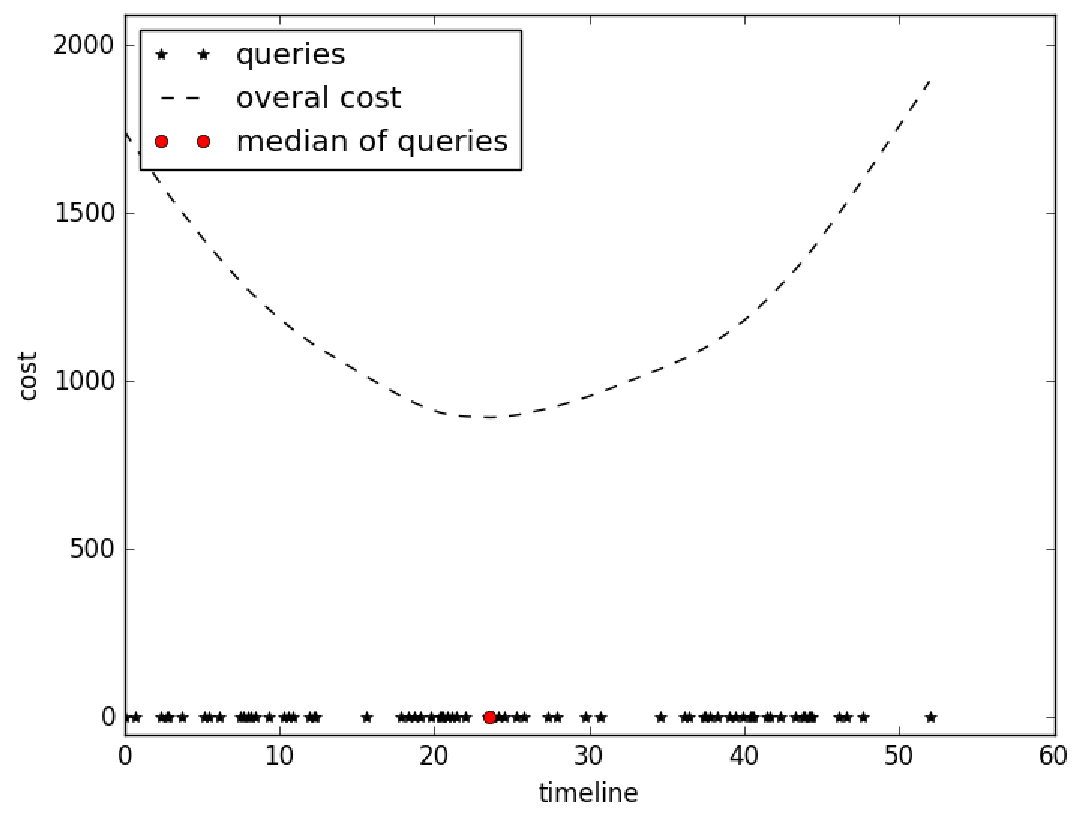
\includegraphics[width=3in]{figs/single.pdf}
    \caption{Cost of query answering using a single snapshot over different
    snaptshot timestamps}
\end{figure}

\begin{figure}[tb]
    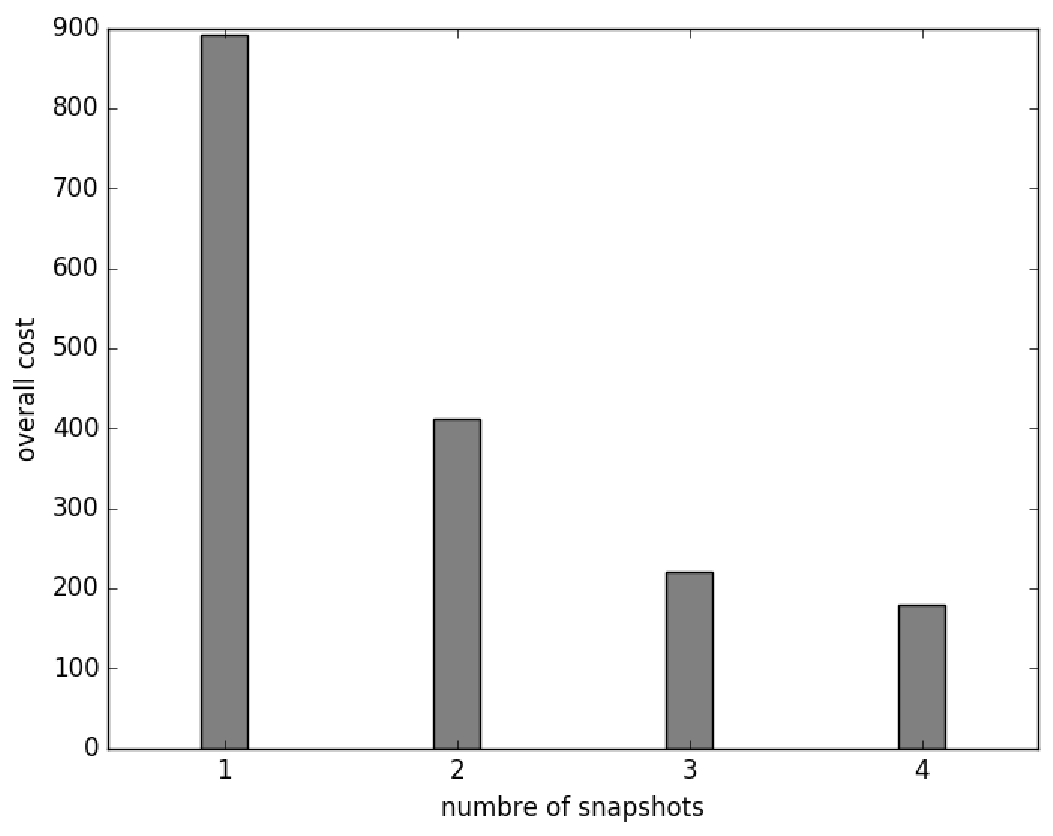
\includegraphics[width=3in]{figs/snap_cost.pdf}
    \caption{Query answering cost with increasing number of snapshots}
\end{figure}
